\subsection{Telemetry Module}

\begin{figure}[H]
\centering
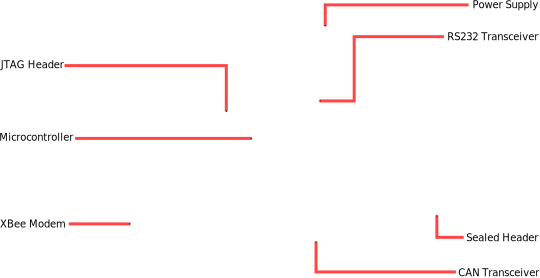
\includegraphics[scale=1]{implementation/figures/telemetry_pcb.eps}
\caption{Populated telemetry module PCB.}\label{fig:telemetry_pcb}
\end{figure}


\begin{figure}[H]
\centering
\def\antenna{
  -- +(0mm,4.0mm) -- +(2.625mm,7.5mm) -- +(-2.625mm,7.5mm) -- +(0mm,4.0mm)
}

\begin{tikzpicture}[auto, node distance=4cm, draw=black!70, >=stealth']
  \node [block, name=max3100] {Max3100 SPI UART};
  \node [block, name=at90, right of=max3100] {AT90CAN};
  \node [block, name=rs232, right of=at90] {Max232 RS232 Transceiver};
  
  \node [block, name=can, below of=at90, above=1cm] {MCP2551 CAN Transceiver};
  \node [block, name=modem, left of=can] {XBee Modem};
  
  \node [block, name=ecu, right of=rs232] {ECU};
  \node [block, name=dac, below of=ecu, above=1cm] {DAC};

  \path (at90.north)+(0.0,+0.4) node (title) {Telemetry Module};

   \begin{pgfonlayer}{background}
       \path (max3100.north west)+(-0.3,0.7) node (a) {};
       \path (can.south -| rs232.east)+(+0.3,-0.2) node (b) {};
       \path[module] (a) rectangle (b);
   \end{pgfonlayer}

  \node [bus, name=can1, below of=can, label=below:CAN Bus, above=2.5cm] {CAN Bus};
  \node [bus, name=can2, left of=can1] {};
  \node [bus, name=can3, right of=can1] {};

  \draw [-, thick] (modem.west) -| ($(modem.west)+(-0.8,0.2)$) \antenna;

  \draw [-, line width=3pt] (can) -- (can1);
  \draw [-, line width=3pt] (can1) -- (can2);
  \draw [-, line width=3pt] (can1) -- (can3);

  \draw [<->, thick] (at90) -- node[] {SPI} (max3100);
  \draw [<->, thick] (max3100) -- node[text width=2cm] {Serial} (modem);
  \draw [<->, thick] ($(at90.east)+(0,0.1)$) to[myncbar, arm=1cm] ($(rs232.north west)+(0,-0.5)$);
  \draw [<-, thick] ($(at90.east)+(0,-0.1)$) to[myncbar, arm=1cm] ($(rs232.south west)+(0,+0.5)$);

  \draw [<->, thick] ($(rs232.north east)+(0,-0.5)$) to[myncbar, arm=1cm] (ecu);
  \draw [<-, thick] ($(rs232.south east)+(0,0.5)$) to[myncbar, arm=1cm] (dac);

  \draw [<->, thick] (at90) -- (can);

%  \draw [<->, thick] (modem) -- node[] {} (telemetry);
%  \draw [<->, thick] (telemetry) -- node[] {RS232} (ecu);
%  \draw [<->, thick] (telemetry) -- node[] {RS232} (daq);
%  \draw [-, thick] (modem) -- node[text width=1.5cm] {} (ant) \antenna;
\end{tikzpicture}
\caption{Block Diagram, Wireless Telemetry Module.\label{fig:tele_tx_overview}}
\end{figure}

The telemetry module is implemented on a custom PCB with the same AT90CAN128 micro-controller common to the other modules. In addition to the common life-support hardware, the telemetry module includes a dual RS-232 transceiver chip and two DE-9 connectors. 

The ECU and the DAQ connect to the telemetry board with specialized cables that connect to the wiring harness. The ECU and DAQ interface with two built-in USART ports on the micro-controller. A third, SPI-based UART interfaces with the wireless transmitter.

\begin{table}[H]
  \caption{Wireless Telemetry Module Components\label{tab:telmetry_module_components}}
  \centering
    \begin{tabular}{|c|c|c|}
      \hline 
      Part & Manufacturer & Part Number\tabularnewline
      \hline
      \hline
      XBee-PRO OEM Module & Digi International & XBee-PRO\tabularnewline
      \hline 
      Dual RS-232 Transceiver & Maxim Electronics & MAX232\tabularnewline
      \hline 
      SPI-capable UART chip & Maxim Electronics & MAX3100\tabularnewline
      \hline 
      300mA Low Dropout Regulator & Linear Technology & LT1521\tabularnewline
      \hline
      8-bit dual-supply level translator & ST Microelectronics & ST2378E\tabularnewline
      \hline
    \end{tabular}
\end{table}


\subsubsection{XBee-PRO Wireless Modem}

To meet the range and data throughput requirements for the telemetry system, an XBee-PRO wireles modem was used. The XBee requires \unit{3.3}{\volt} I/O levels and power supply, and so a second linear voltage regulator was used in the design, the LT1521 from Linear Technology. Since the AT90CAN129 has only 2 built-in UARTS that were used for the RS232 interfaces to the ECU and DAQ, an third external UART was added to the design. The MAX3100 is a SPI-interfaced UART with an 8 word deep FIFO buffer. It is interfaced to the AT90CAN128's SPI pins and has an active-low IRQ line connected to external interrupt line EXT7 on the microcontroller. 

The wireless transmitter is an XBee Pro Modem from Digi International. The modem is in a package designed for mounting on a printed circuit board, and is attached to the telemetry module directly. This modems requires a 3.3V power supply. and consumes at most 215mA of current during transmit. Since the common module hardware only provides power for 5V devices, the telemetry module has a second LDO regulator providing 3.3V. A separate antenna port is connected to the modem and mounted in the side of the module enclosure.

\subsubsection{Dual RS-232 Transceiver}

A MAX232 dual RS-232 trasceiver chip was used in the design to interface the built-in UARTS on the AT90CAN128 with the line levels expected by the serial ports on the ECU and DAQ.

\subsubsection{External SPI USART}

A third UART was needed in the design to interface with the XBee-PRO modem, since the AT90CAN128 only provides 2. A MAX3100 SPI-capable external UART was chosen


\subsubsection{Two-Channel ECU and DAC USART}